% !TEX root = 99_main.tex

\subsection{Sensitivity of the Building Envelope}
\label{ch:envelope}

Figure \ref{fig:envelopeASF} details the performance of the ASF constructed on a typical office building with respect to the envelope U-value. As expected the heating demand increases with increasing U-value. Interestingly, the photovoltaic electricity supply decreases. This is because the ASF always optimises for net energy minimisation. With increasing heating demands, the ASF will optimise for positions that direct solar radiation into the building to minimise the heating loads as opposed to generating the electricity on the panels. This same characteristic is apparent in \ref{fig:envelopecompNo} which compares the energy saving potential of the ASF compared to a glazed facade with no shading system. A building with low envelope U-value will have a large saving potential due to the reduction of cooling loads, and supply of photovoltaic electricity. As the envelope U-value increases, this saving potential begins to decrease.

Figure \ref{fig:envelopecompstatic} compares the ASF to an equivalent static photovoltaic shading system with panels orientated in the most energetically favourable position. As the U-value increases the net energy saving increases. As mentioned earlier, the heating demand increases with increasing U-value. For high U-value envelopes, the ASF will adapt and open up the panels thus reducing the heating demands. The equivalent static system will remain in a semi closed position for the entire year, and will block the solar heat gains necessary in winter.

Figure \ref{fig:infiltration} details the equivalent analysis with varying infiltration rates. Similar trends can be observed to those in Figure \ref{fig:envelope}. Leakier buildings lead to high heat demands, which decreases the performance of the ASF compared to a glazed window with no shading, but increases the performance relative to a static shading system. 



\begin{figure}
    \centering
    \begin{subfigure}[b]{0.47\textwidth}
        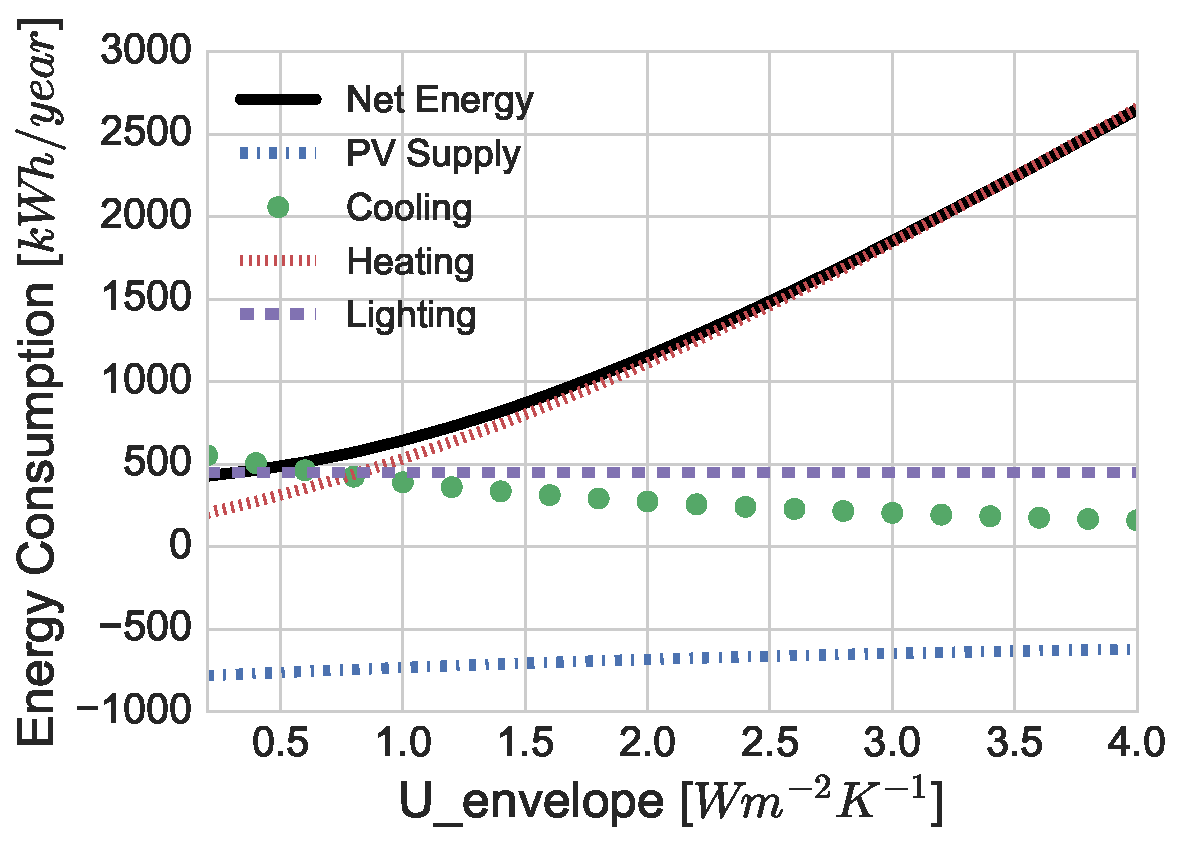
\includegraphics[width=\textwidth]{Sensitivity_ZH_U_env_COP3_1_ASF.pdf}
        \caption{} 
        \label{fig:envelopeASF} 
    \end{subfigure} \vfill
    \begin{subfigure}[b]{0.47\textwidth}
        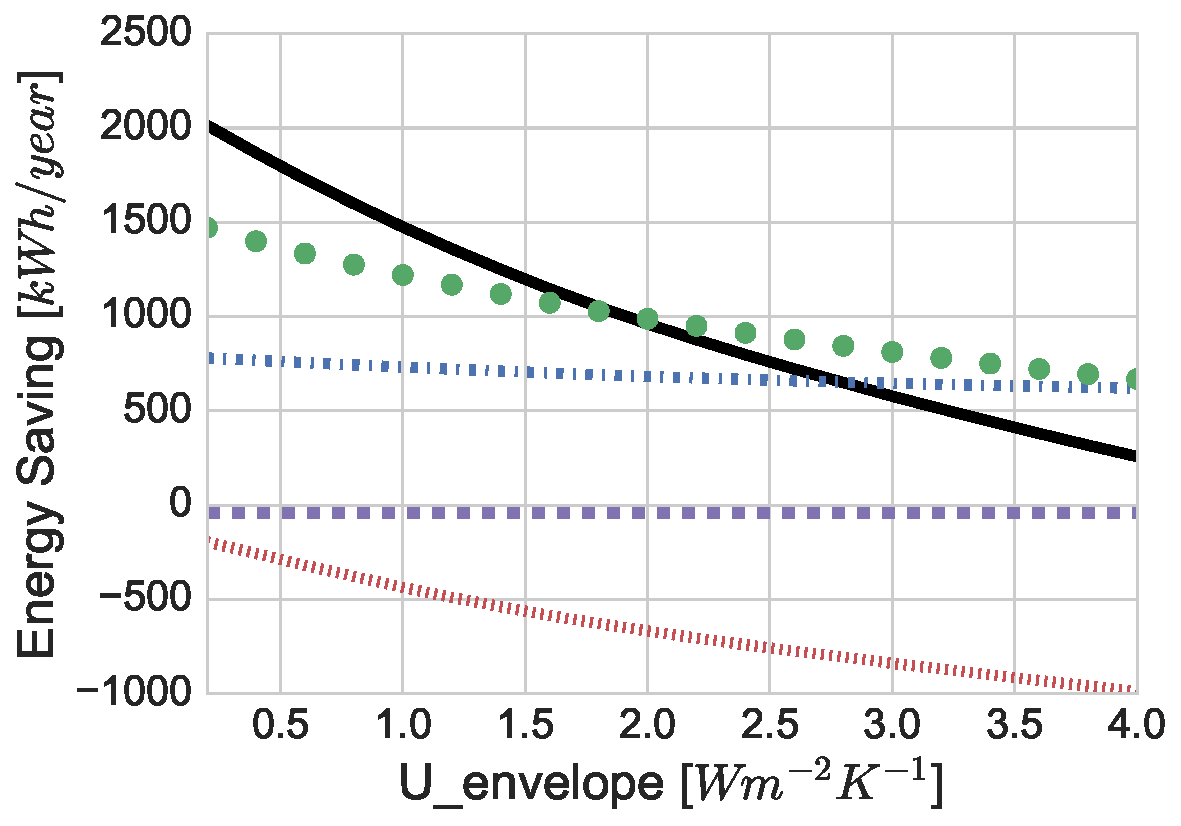
\includegraphics[width=\textwidth]{Sensitivity_ZH_U_env_COP3_1EnergySavingNoASF.pdf}
        \caption{}
        \label{fig:envelopecompNo} 
    \end{subfigure} \hfill
    \begin{subfigure}[b]{0.47\textwidth}
        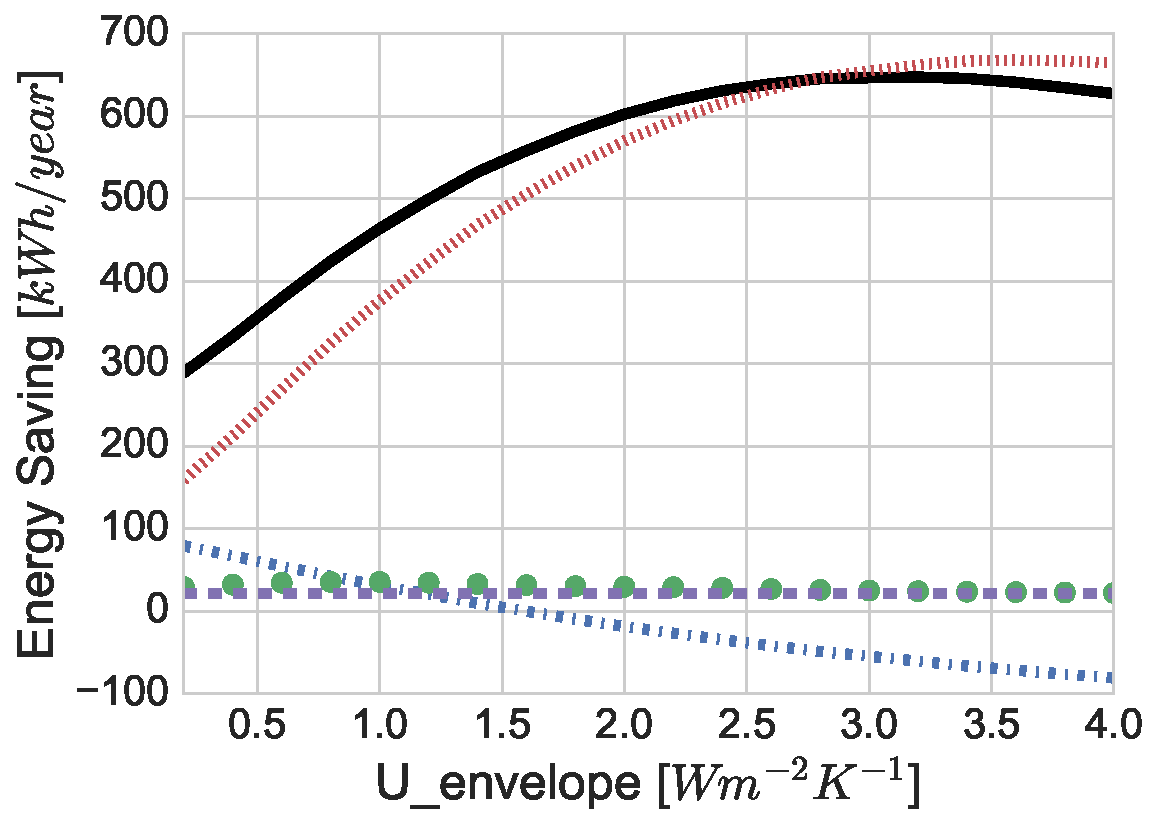
\includegraphics[width=\textwidth]{Sensitivity_ZH_U_env_COP3_1EnergySavingStatic.pdf}
        \caption{}
        \label{fig:envelopecompstatic} 
    \end{subfigure} 
    
    \caption{Influence of envelope thermal transmittance (U-value). a) Details the energetic performance of the ASF with respect to building envelope U-value. b) compares the energy saving potential of an ASF relative to a facade with no shading system. c) compares the energy saving potential of an ASF relative to an equivalent static PV system. }
    \label{fig:envelope}
\end{figure}


\begin{figure}
    \centering
    \begin{subfigure}[b]{0.47\textwidth}
        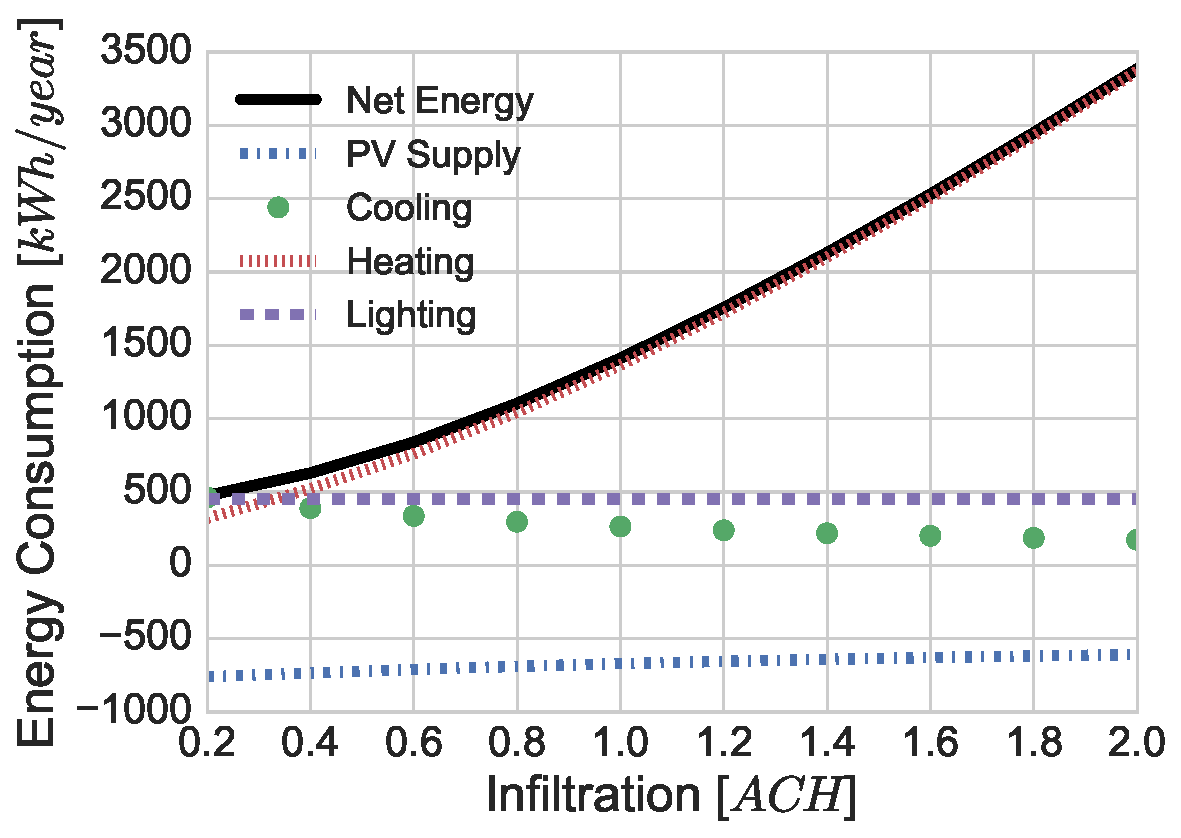
\includegraphics[width=\textwidth]{Sensitivity_ZH_Infl_COP3_1_ASF.pdf}
        \caption{} 
        \label{fig:infiltrationASF}
    \end{subfigure} \vfill
    \begin{subfigure}[b]{0.47\textwidth}
        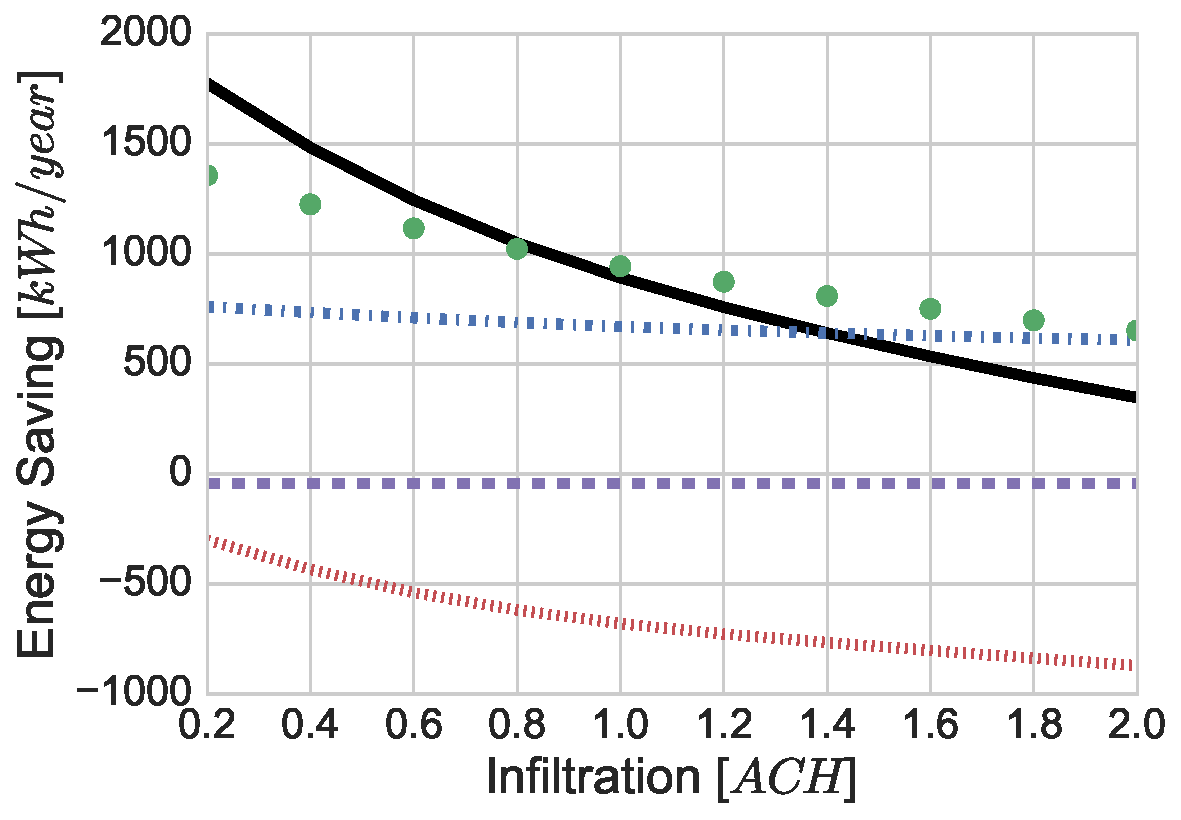
\includegraphics[width=\textwidth]{Sensitivity_ZH_Infl_COP3_1EnergySavingNoASF.pdf}
        \caption{}
        \label{fig:infiltrationcompNo}
    \end{subfigure}\hfill
    \begin{subfigure}[b]{0.47\textwidth}
        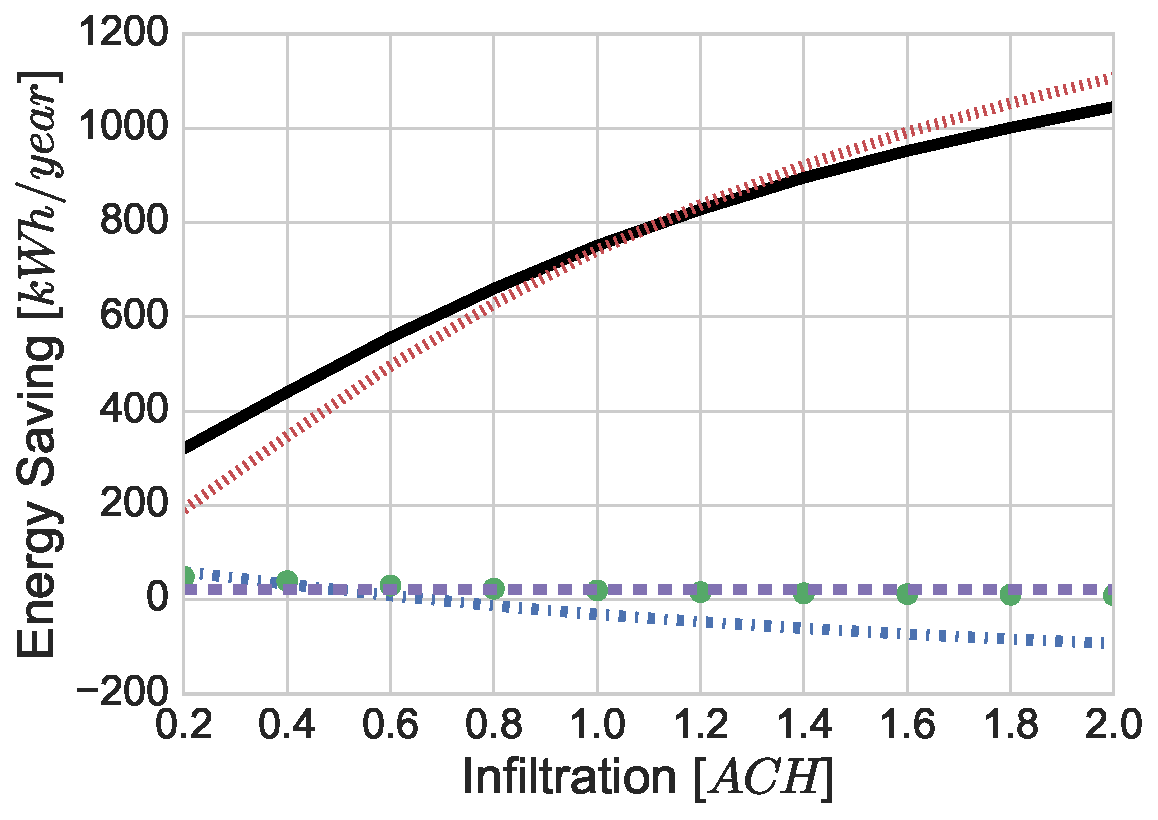
\includegraphics[width=\textwidth]{Sensitivity_ZH_Infl_COP3_1EnergySavingStatic.pdf}
        \caption{}
        \label{fig:infiltrationcompstatic}
    \end{subfigure}
    \hfill
    \caption{Influence of infiltration. a) Details the energetic performance of the ASF with respect to building infiltration. b) compares the energy saving potential of an ASF relative to a facade with no shading system. c) compares the energy saving potential of an ASF relative to an equivalent static PV system.}
    \label{fig:infiltration}
\end{figure}


\subsection{Archetype Evaluation of the ASF}

Figure \ref{fig:ArchResultsNoASF} compares the energy saving potential of 11 building use types with six different construction periods compared to a glazed facade with no shading system. Darker colours indicate larger energy saving potentials. One clear trend is the increasing saving potential in newer buildings over older buildings. This can be attributed to the lower envelope U-value in newer buildings, which as discussed in Section \ref{ch:envelope} will increase the energy saving potential. It is also interesting to note that the ASF performs best in gym use types. Gyms have a large cooling demand due to the high human heat emissions. Optimum configurations for cooling minimisation generates the maximum photovoltaic electricity supply. 


However, an ASF is not necessarily the best design solution for buildings with a large cooling demand. Figure \ref{fig:ArchResultsStatic} compares the ASF performance against an equivalent static system. If we once again focus on the modern gym, we notice that there is only a small increase in the energy performance of an adaptive system over an optimally configured static system. When comparing both heat maps we see that an ASF performs best on in a modern office, retail store, food store, and school. These archetypes perform well due to two reasons. Firstly, they have an even balance of heating and cooling demands. Thus there is a need for adaptivity in the envelope to reduce these demands. Secondly, these archetypes are in use during the day. Residential buildings on the other hand are mostly occupied at night where the ASF has no influence on the building performance.

\begin{figure}
\begin{center}
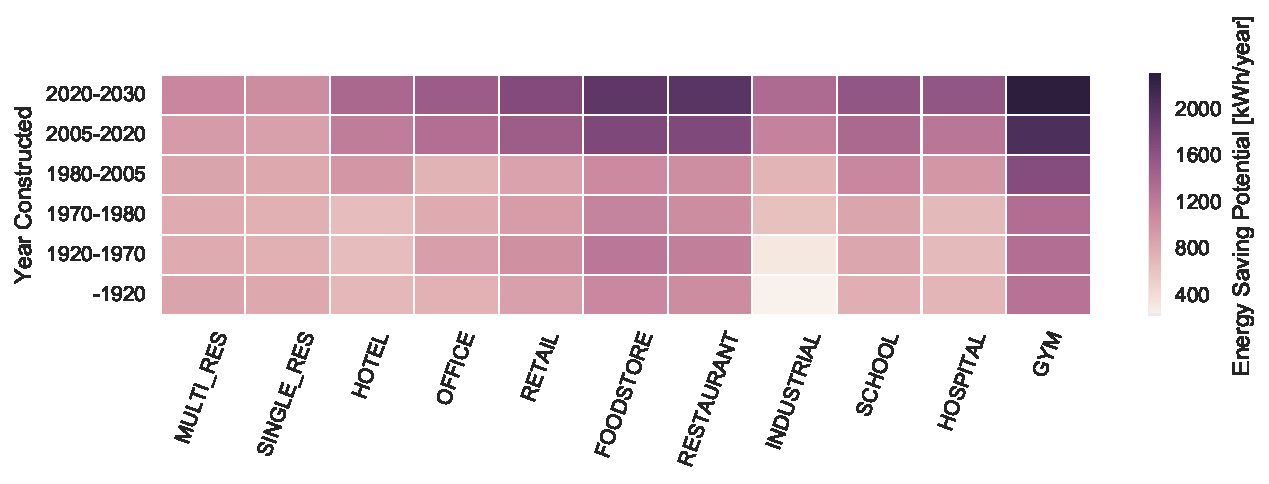
\includegraphics[width=\textwidth, trim= 0cm 0cm 0cm 0cm,clip]{energySaving_COP1_3_NoASF.pdf}
\caption{Annual results detailing the energy saving potential of the ASF vs a glazed window with no shading system}
\label{fig:ArchResultsNoASF}
\end{center}
\end{figure}

\begin{figure}
\begin{center}
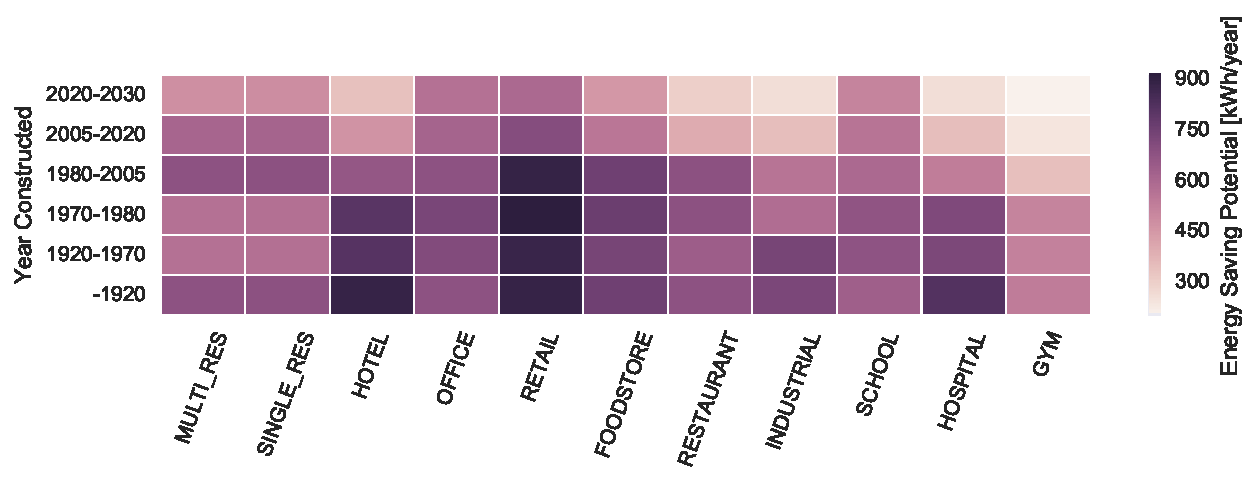
\includegraphics[width=\textwidth, trim= 0cm 0cm 0cm 0cm,clip]{energySaving_COP1_3_static.pdf}
\caption{Annual results detailing the energy saving potential of the ASF vs a static photovoltaic shading system}
\label{fig:ArchResultsStatic}
\end{center}
\end{figure}